% TODO: this document is **highly** based on a RoboCup document from 2010 with
% no indication on the authors, however, there should be citation or at least
% some credits
\clearpage
\sffamily
{\bfseries\color[rgb]{0.4,0.4,0.4} Center of mass measurement}
\phantomsection
\addcontentsline{toc}{subsection}{Center of mass measurement}

\bigskip

This sections presents the official procedure to measure $H_{COM}$,
the height of the center of mass of the robot used in Law 4.
It also provides instructions on how to build the measuring device used in the
procedure.

\bigskip

{\bfseries Construction of the measuring device}

\headlinebox

The dimensions of the device are different for KidSize and AdultSize.
In this section, $H_{max}$ denotes the maximum height allowed for the
according league (100cm for KidSize, 200cm for AdultSize).
$W$ denotes the width of the measuring device (45cm for KidSize, 80cm for
AdultSize).
% TODO: Values of W needs to be adjusted/agreed on.
% - The 45cm for KidSize had been chosen when H_{max} was 60cm.
%   - One example of robot: Htop=70cm,W=30cm -> (9cm margin including acrylic plates)
% - The 80cm is just a wild guess not supported by any data

\bigskip

\textbf{The required materials are:}
\begin{itemize}
\item 1 measuring tape of length $H_{max}$
\item An aluminium plate ($H_{max}+5cm$ by $39cm$)
\item A wooden board - Plywood ($H_{max}+20cm$ by $W$ by $1.5cm$)
  % TODO: 1.5cm of wood is probably insufficient for the heaviest robot of
  % AdultSize (50kg)
  % TODO: Should the +20cm scale up? Initial understanding is that the device
  % can be used if: abs(H_com - H_top/2) < 20cm/2 + (H_max - H_top)
  % This might be problematic for 2m height robot which would need to have Hcom
  % in [90cm,110cm] (while the rule allows a much larger range since the only
  % constraint is the size of the foot)
\item Two acrylic plates ($H_{max}$ by 3cm by 2-3 mm)
  % TODO: fig:gluing-acrylic-plates show that the dimension is rather $H_{max}+20cm$
\item 4 Aluminium pipe straps of same size
\end{itemize}

\textbf{Steps for building the measuring device}
\begin{enumerate}
\item Glue two acrylic plate on each side of the wooden board as shown in
  Fig~\ref{fig:gluing-acrylic-plates}.
\item Draw a white line on the middle of the board, over the acrylic plates.
\item Screw 4 aluminimum pipe straps at the back-middle of the wooden board,
aligning horizontally as shown in Fig~\ref{fig:aligning-pipe-straps}.
This is to determine whether the robot weight is balanced.
\item Bend 4cm of the aluminimum plate to 90 degrees and tape the $H_{max}$
  measuring tape as shown in Fig~\ref{fig:bending-aluminium-plate}.
\end{enumerate}

\begin{figure}[htb]
  \centering
  \begin{subfigure}{.45\textwidth}
    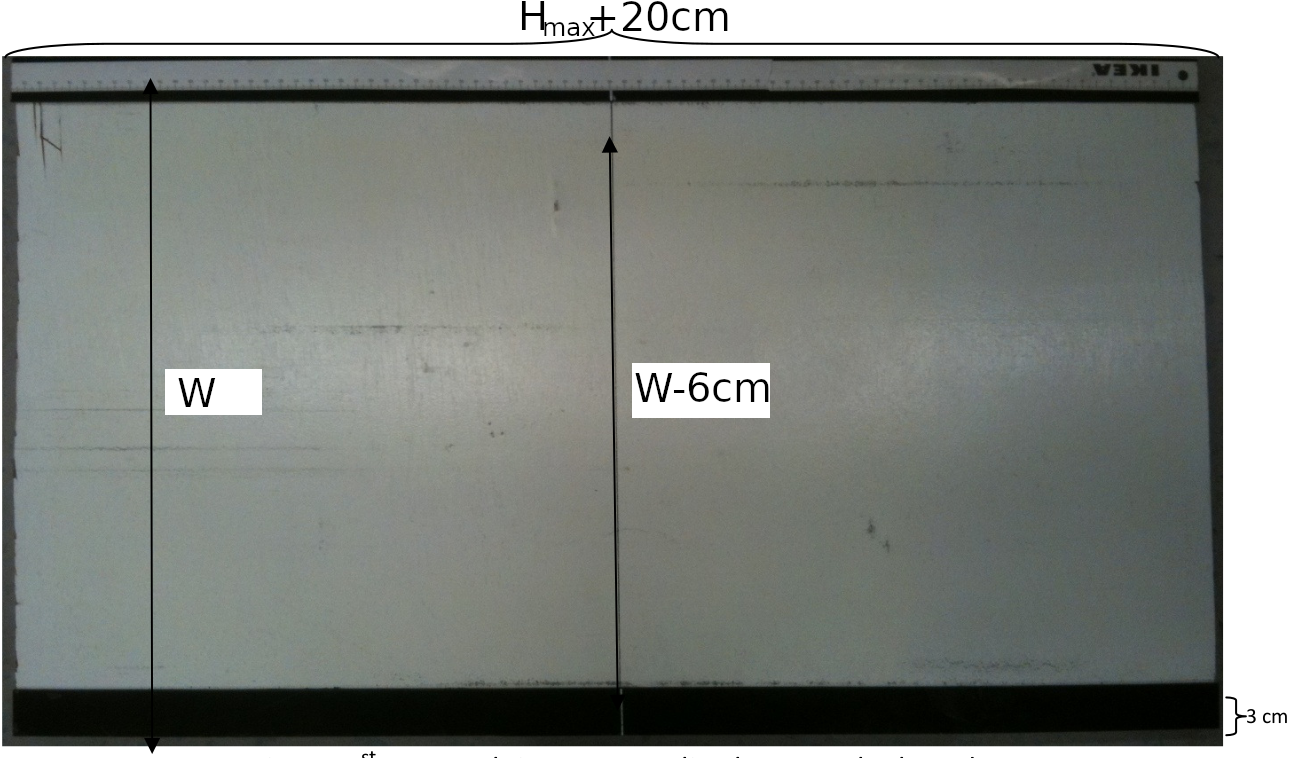
\includegraphics[width=\textwidth]{img/com-device-step1}
    \caption{Gluing two acrylic plates on the wooden board}
    \label{fig:gluing-acrylic-plates}
  \end{subfigure}
  \hfill
  \begin{subfigure}{.45\textwidth}
    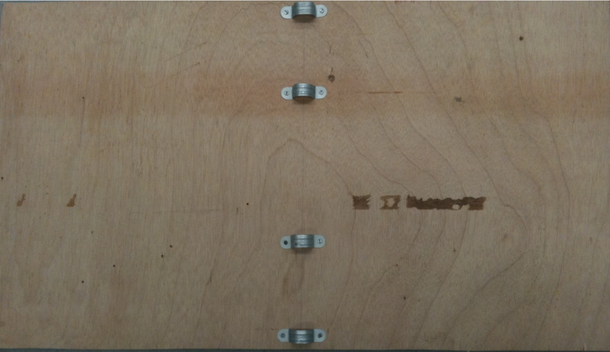
\includegraphics[width=\textwidth]{img/com-device-step2}
    \caption{Aligning pipe straps on the wooden board}
    \label{fig:aligning-pipe-straps}
  \end{subfigure}
  \begin{subfigure}{.45\textwidth}
    \centering
    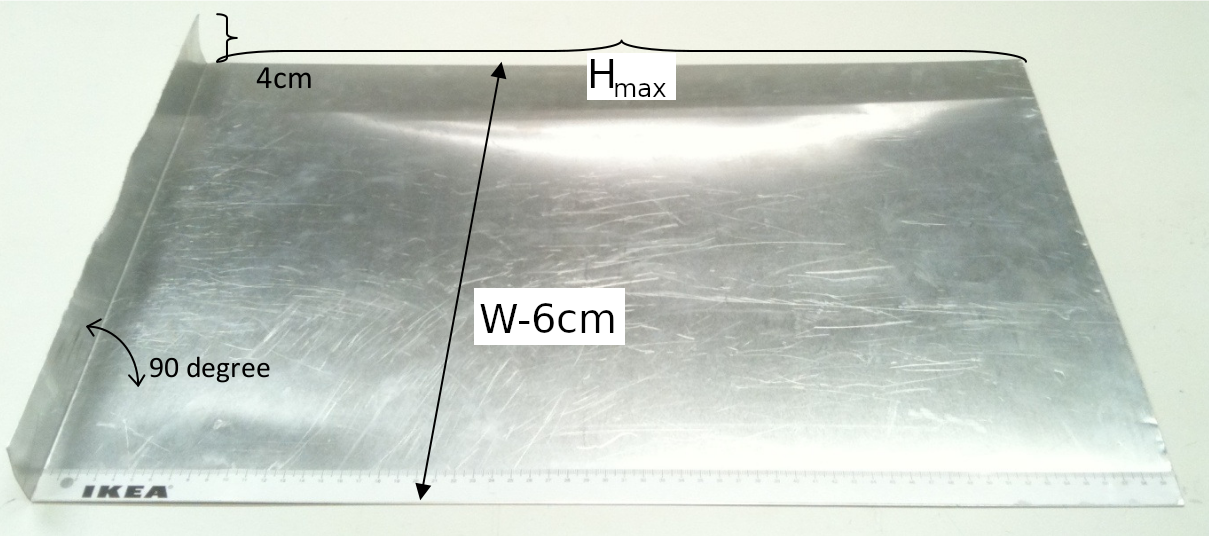
\includegraphics[width=\textwidth]{img/com-device-step3}
    \caption{Bending the aluminimum plate}
    \label{fig:bending-aluminium-plate}
  \end{subfigure}
  \caption{Building the measuring device for $H_{COM}$}
\end{figure}

\bigskip

{\bfseries Measuring the center of mass}

\headlinebox

\begin{enumerate}
\item Place the robot flat onto the aluminium plate holding,
  touching the bottom of the bended aluminium plate.
\item Ensure that the robot is in an upright pose\footnote{see
    Fig~\ref{fig:bodyplan}, in Law 4}
  as shown in Fig~\ref{fig:com-measurement-1}.
\item Align the metal frame holding with the wooden board as shown in
  Fig~\ref{fig:com-measurement-2}.
\item Slowly, slide the aluminium plate to towards the other end until the
  wooden board is balanced as shown in Fig~\ref{fig:com-measurement-3}.
\item Record the reading shown by the white line in the middle of the wooden
  board pointing to the measuring tape,
  as shown in Fig~\ref{fig:com-measurement-4}.
\end{enumerate}

\begin{figure}
  \begin{subfigure}{.45\textwidth}
    \centering
    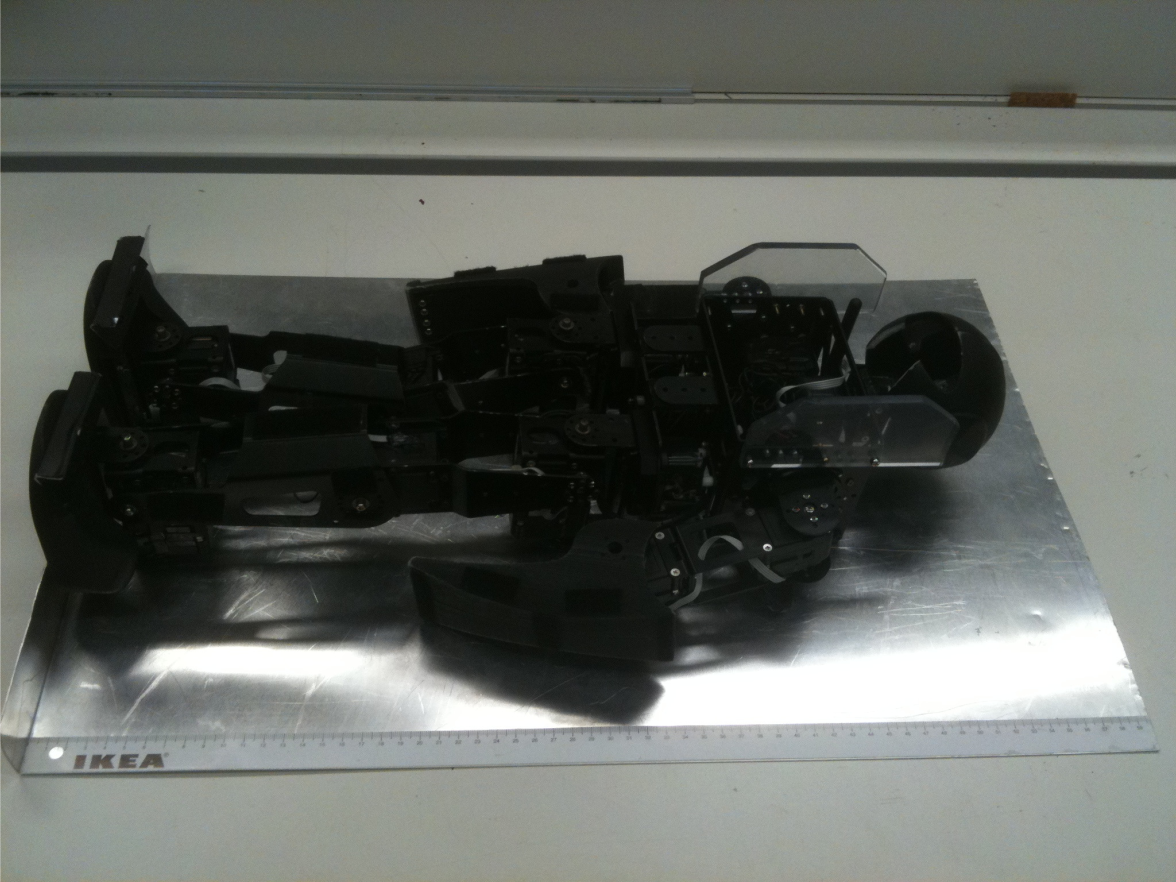
\includegraphics[width=\textwidth]{img/com-measurement-step1}
    \caption{Laying robot upright on measurement device.}
    \label{fig:com-measurement-1}
  \end{subfigure}
  \hfill
  \begin{subfigure}{.45\textwidth}
    \centering
    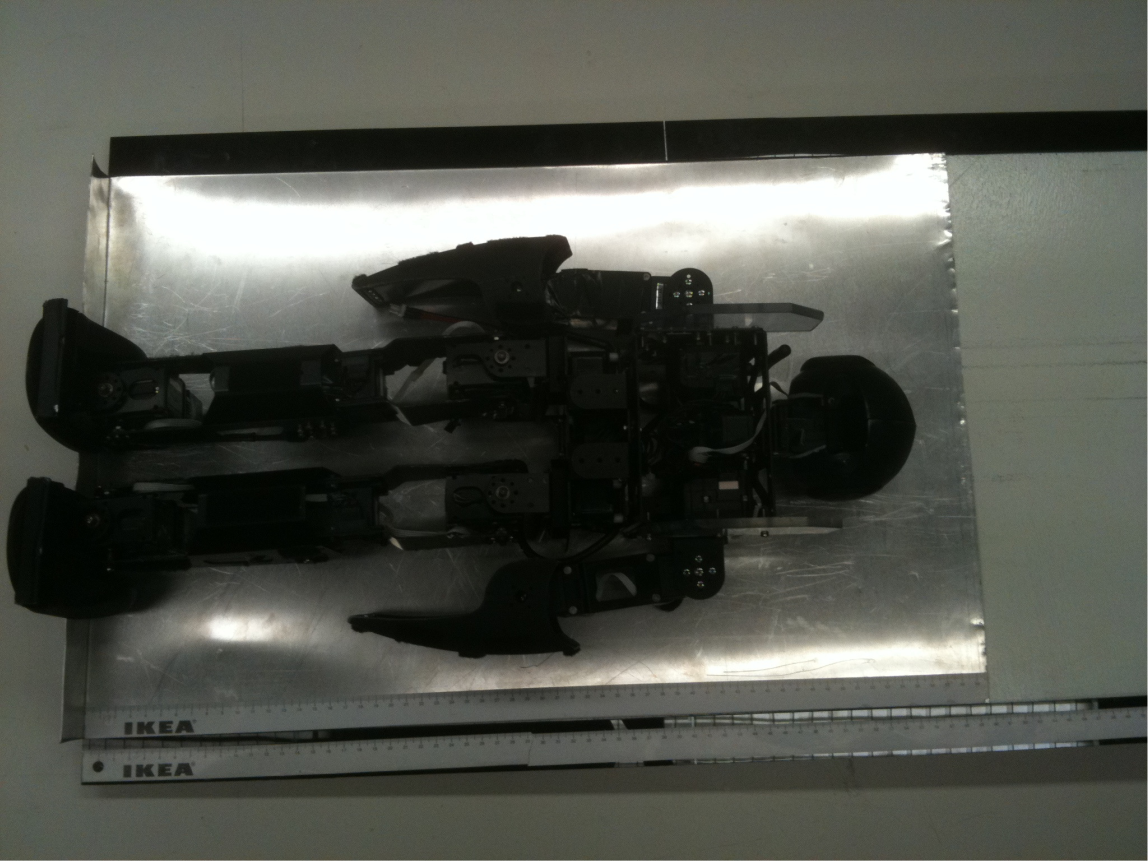
\includegraphics[width=\textwidth]{img/com-measurement-step2}
    \caption{Aligning metal frame holding with wooden board.}
      \label{fig:com-measurement-2}
  \end{subfigure}
  \\
  \begin{subfigure}{.45\textwidth}
    \centering
    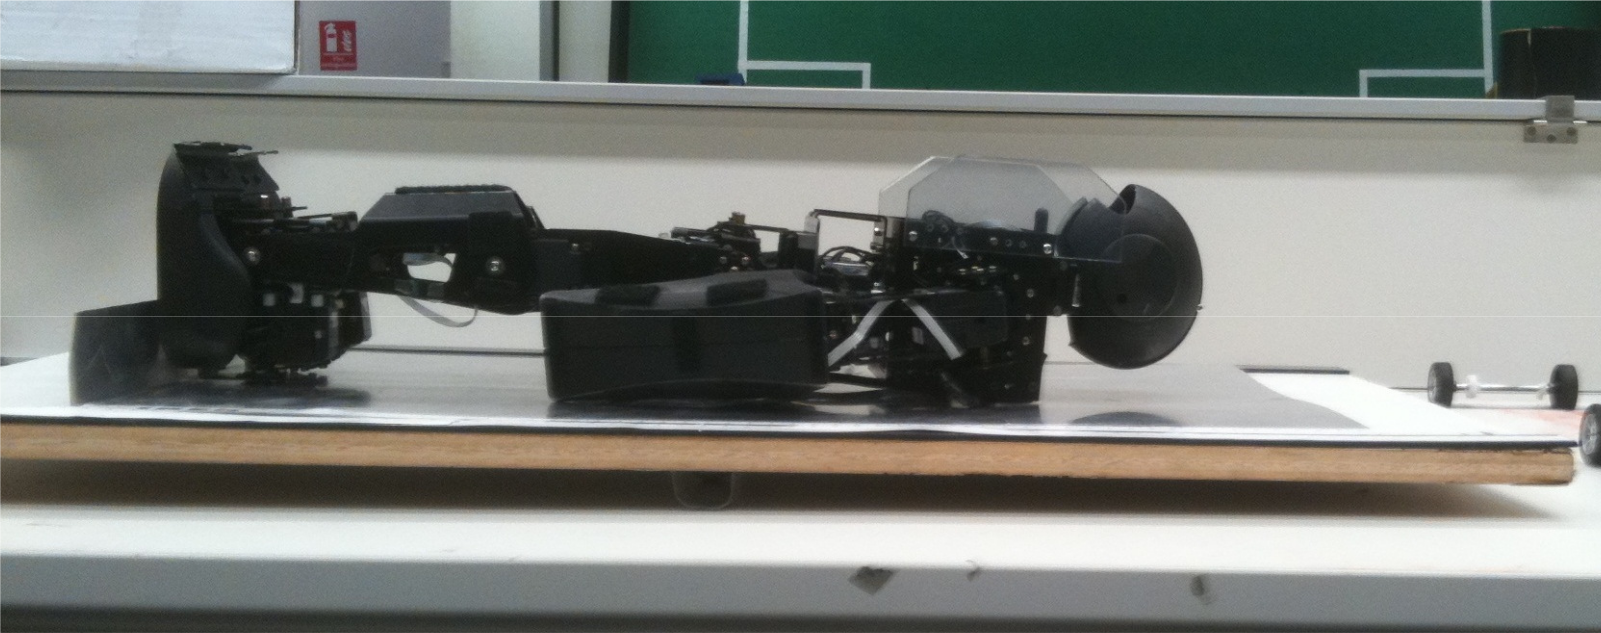
\includegraphics[width=\textwidth]{img/com-measurement-step3}
    \caption{Balancing the wooden board by sliding the aluminium plate.}
    \label{fig:com-measurement-3}
  \end{subfigure}
  \hfill
  \begin{subfigure}{.45\textwidth}
    \centering
    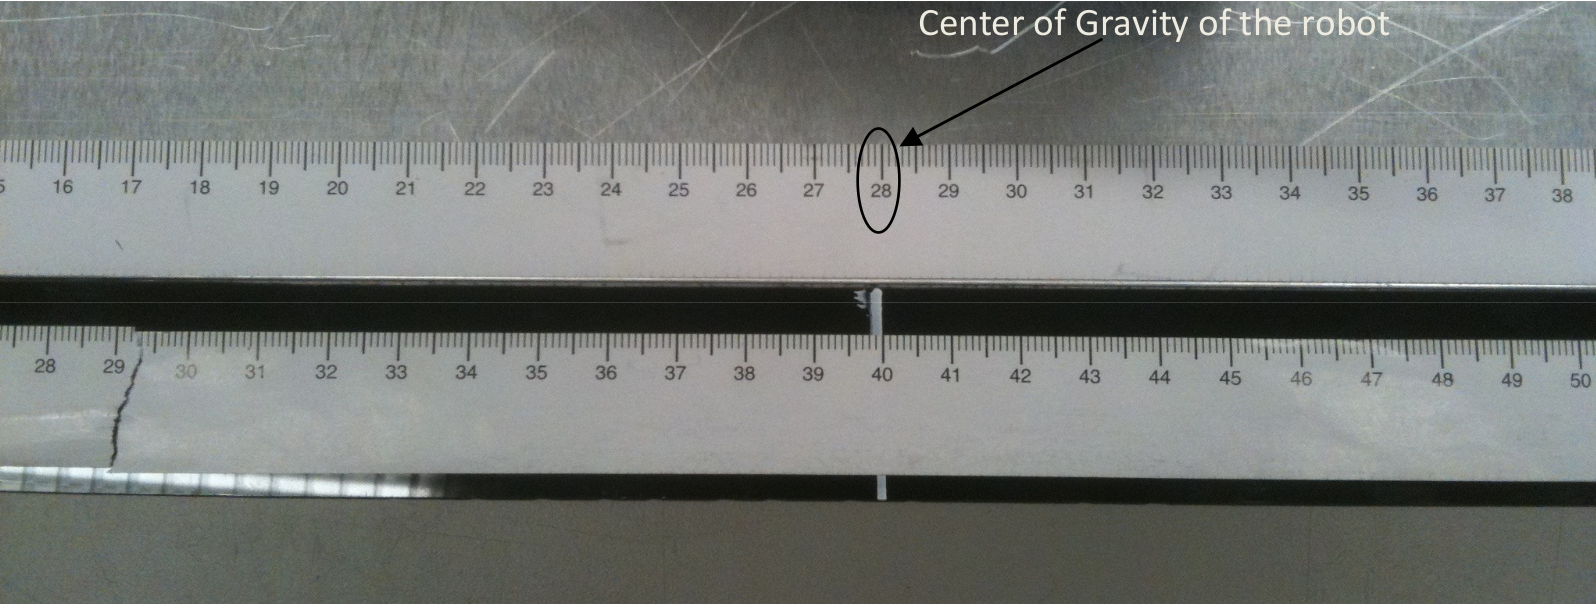
\includegraphics[width=\textwidth]{img/com-measurement-step4}
    \caption{Reading $H_{COM}$ on the device}
    \label{fig:com-measurement-4}
  \end{subfigure}
  \caption{Procedure for measuring $H_{COM}$}
\end{figure}